%----------------------------- LE CLIENT ----------------------------- 
\subsection{Le client}

% Logo Eirlab
\begin{center}

\includegraphics[scale=0.11]{img/eirlab_logo.png}
\end{center}

Ce projet est initié par Eirlab, le FabLab de l'ENSEIRB-MATMECA/Bordeaux INP. Il s'agit d'un atelier de fabrication numérique mettant à disposition de ses membres des outils de prototypage rapide. Les locaux de l'atelier se trouvent dans l'école ENSEIRB-MATMECA, à Talence.

L'atelier a ouvert au printemps 2016, il est plus particulièrement régi par l'association Eirlab Community. Cette dernière a pour objet la gestion, l'animation et la promotion de l'espace Eirlab à travers des évènements, formations gratuites ou payantes. L'association propose également un service de vente de matériaux pour les réalisations.

Peuvent adhérer au club personnes physiques, étudiantes de Bordeaux INP ou non, et personnes morales. 

Eirlab dispose de 400m² d'espace \textit{innovation} d'une part avec des stations de travail, et espaces de discussion, et espace de \textit{prototypage} d'autre part. Ce dernier met à disposition de ses membres six imprimantes 3D, une machine de découpe et gravure laser, une perceuse colonne, et autres outils électroniques et mécaniques. 

Le client est représenté par M. David RENAULT, comme initiateur du projet et principal interlocuteur pour les prises de décisions et validation du travail accompli. 


%----------------------------- LE BESOIN ----------------------------- 
\subsection{Description du besoin}

Le projet se place dans le cadre de l'utilisation de la machine de découpe/gravure laser pour usiner des pièces en deux dimensions.

\subsubsection*{Description de l'existant}

\begin{wrapfigure}{r}{6cm}
    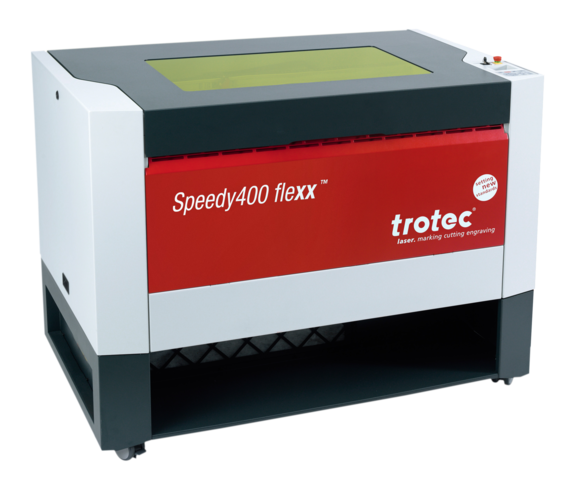
\includegraphics[scale=0.3]{img/lasermachine.png}
    \caption{Machine laser 400 Flexx Trotec}
    \label{fig:lasermachine}
\end{wrapfigure}

La machine présente à l'atelier est le modèle 400 Flexx de Trotec, elle permet de graver de nombreux matériaux, et de découper ou marquer certains d'entre eux. 

L'envoi de travaux à la machine se fait depuis le poste de travail à côté de celle-ci, depuis le logiciel de conception en passant par le logiciel de contrôle d'impression propriétaire \textit{JobControl}. L'usage à Eirlab est d'utiliser le logiciel \textit{Inkscape} pour éditer les fichiers vectoriels SVG à découper/graver.


\subsubsection*{Besoins du client}
Afin d'optimiser le temps de découpe et d'économiser les matériaux, le client souhaite faire intervenir un algorithme de \textit{packing} avant lancement de la découpe. Il s'agit de calculer une disposition des pièces à découper occupant le moins d'espace possible. Cette étape est pour le moment réalisée manuellement, ce qui est fastidieux pour l'utilisateur, et n'assure pas l'optimalité de l'agencement choisi. Voici un exemple en figure \ref{fig:before_after_pack} fichier source et de résultat attendu :

\begin{figure}[!htb] 
    \centering
    
\includegraphics[scale=0.12]{img/verteall.png}
    \caption{Exemple de packing attendu}
    \label{fig:before_after_pack}
\end{figure}

La figure \ref{fig:schema_besoin} suivante représente les différentes étapes traversées lors de l'utilisation de la découpeuse laser. Notre projet doit donc s'inscrire au niveau de l'étape d'édition du fichier vectoriel dans le logiciel Inkscape. 

\begin{figure}[H]
    \centering
    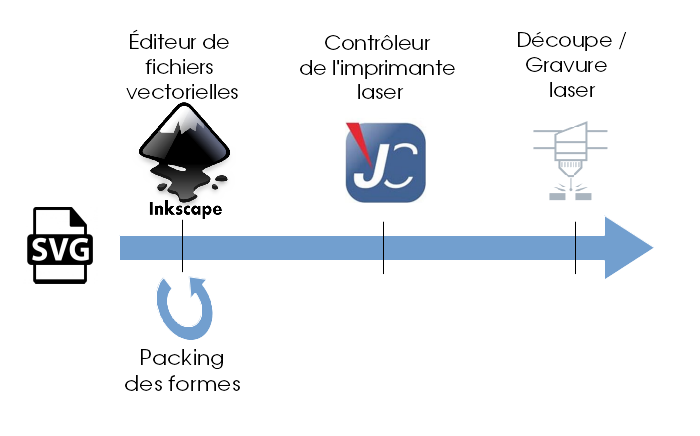
\includegraphics[scale=0.6]{img/schema_besoin.png}
    \caption{Schéma des étapes du cas d'utilisation général souhaité pour la découpe laser}
    \label{fig:schema_besoin}
\end{figure}



%% ------------ LE SUJET ------------ %%

\subsection{Le sujet}

Le client a souhaité que soit fourni un plug-in pour le logiciel Inkscape, depuis lequel il puisse déclencher les fonctionnalités de \textit{packing} développées dans notre solution, en plus de l'application depuis le terminal.

Il nous a été demandé de mettre en place un ensemble d'algorithmes réalisant de différentes manières une solution au problème de \textit{packing}. Ces derniers doivent pouvoir être lancés en parallèle, reprendre la solution de l'un comme entrée de l'autre etc., en somme, garantir une certaine modularité dans leur utilisation.



%Notre tâche première pour répondre aux besoins du client a été d'implémenter une base de solveur qui travaille avec des données vectorielles, avec le plug-in Inkscape associé pour une utilisation facile.

%Une fois les fondations de notre travail bien posées, il a fallu nous attaquer au solveur, qui regroupe des algorithmes de packing.
%Ces algorithmes seront de plus en plus complexes dans le but d'obtenir des résultats les plus efficaces possibles. On note par exemple la différence entre les algorithmes ne s'occupant que de rectangles par opposition à ceux qui gèrent l'imbrication de pièces.

%Il nous faut ensuite optimiser ce solveur afin que les algorithmes soient répartis efficacement sur les divers processeurs de la machine.

\subsubsection{Le problème de Bin-Packing}
La problématique d'optimiser l'espace et le nombre de planches utilisées constitue une instance d'un problème de bin-packing.\\

Le bin-packing est un problème relevant de l'optimisation combinatoire, ou il s'agit de ranger des objets de tailles $c_{1}, c_{2}, ... , c_{n}$ dans le minimum de boites de taille $C$(correspondant à des plaques dans notre cas).\\

Ce problème est présent dans plusieurs secteurs d'activité tels que le rangement de fichier dans un système informatique ou le découpage du verre.

Le problème de Bin-Packing est NP-difficile, donc à part pour les problèmes de tailles très réduites, les méthodes de résolutions sont principalement heuristiques et métaheuristiques.\\

Les méthodes heuristiques les plus utilisées de nos jours sont :  
\begin{itemize}
    \item \textit{first-fit decreasing (FFD)}: qui consiste à trier les objets dans un ordre décroissant de taille, puis pour chaque objet, on le range dans la première boite qui peut le contenir. 
    \item \textit{best-fit decreasing (BFD)}: le même tri qu'auparavant, sauf qu'on range l'objet dans la boîte la plus remplie qui puisse le contenir.
\end{itemize}
~\\

Plusieurs articles et thèses existent pour ce problème se basant sur différentes techniques d'optimisation telle que le branch and bound:\\

\textit{  Two-Dimensional Finite Bin-Packing Algorithms J. O. Berkey and P. Y. Wang The Journal of the Operational Research Society Vol. 38, No. 5 (May, 1987), pp. 423-429  ) }\\

\textit{A Genetic Algorithm for a 2D Industrial Packing Problem E. Hopper, B. Turton University of Wales, Cardiff, Computers and Industrial Engineering, vol. 37/1-2, pp. 375-378, 1999. }\\
